
\documentclass[fleqn,addpoints]{exam}
\usepackage{amsmath}
\usepackage{graphicx}
\usepackage{booktabs}
\usepackage{float}
\usepackage{caption}
\usepackage{polynom}
\usepackage{mdwlist}
\usepackage{cancel}

\usepackage{unitsdef} 
\newunit{\inch}{in}
\newunit{\mile}{mile}
\newunit{\mph}{mph}
\newunit{\foot}{ft}
\newunit{\knot}{knot}
\newunit{\gallon}{gallon}

\bracketedpoints
\everymath{\displaystyle}

\printanswers


% \begin{figure}[H]
%   \centering
%   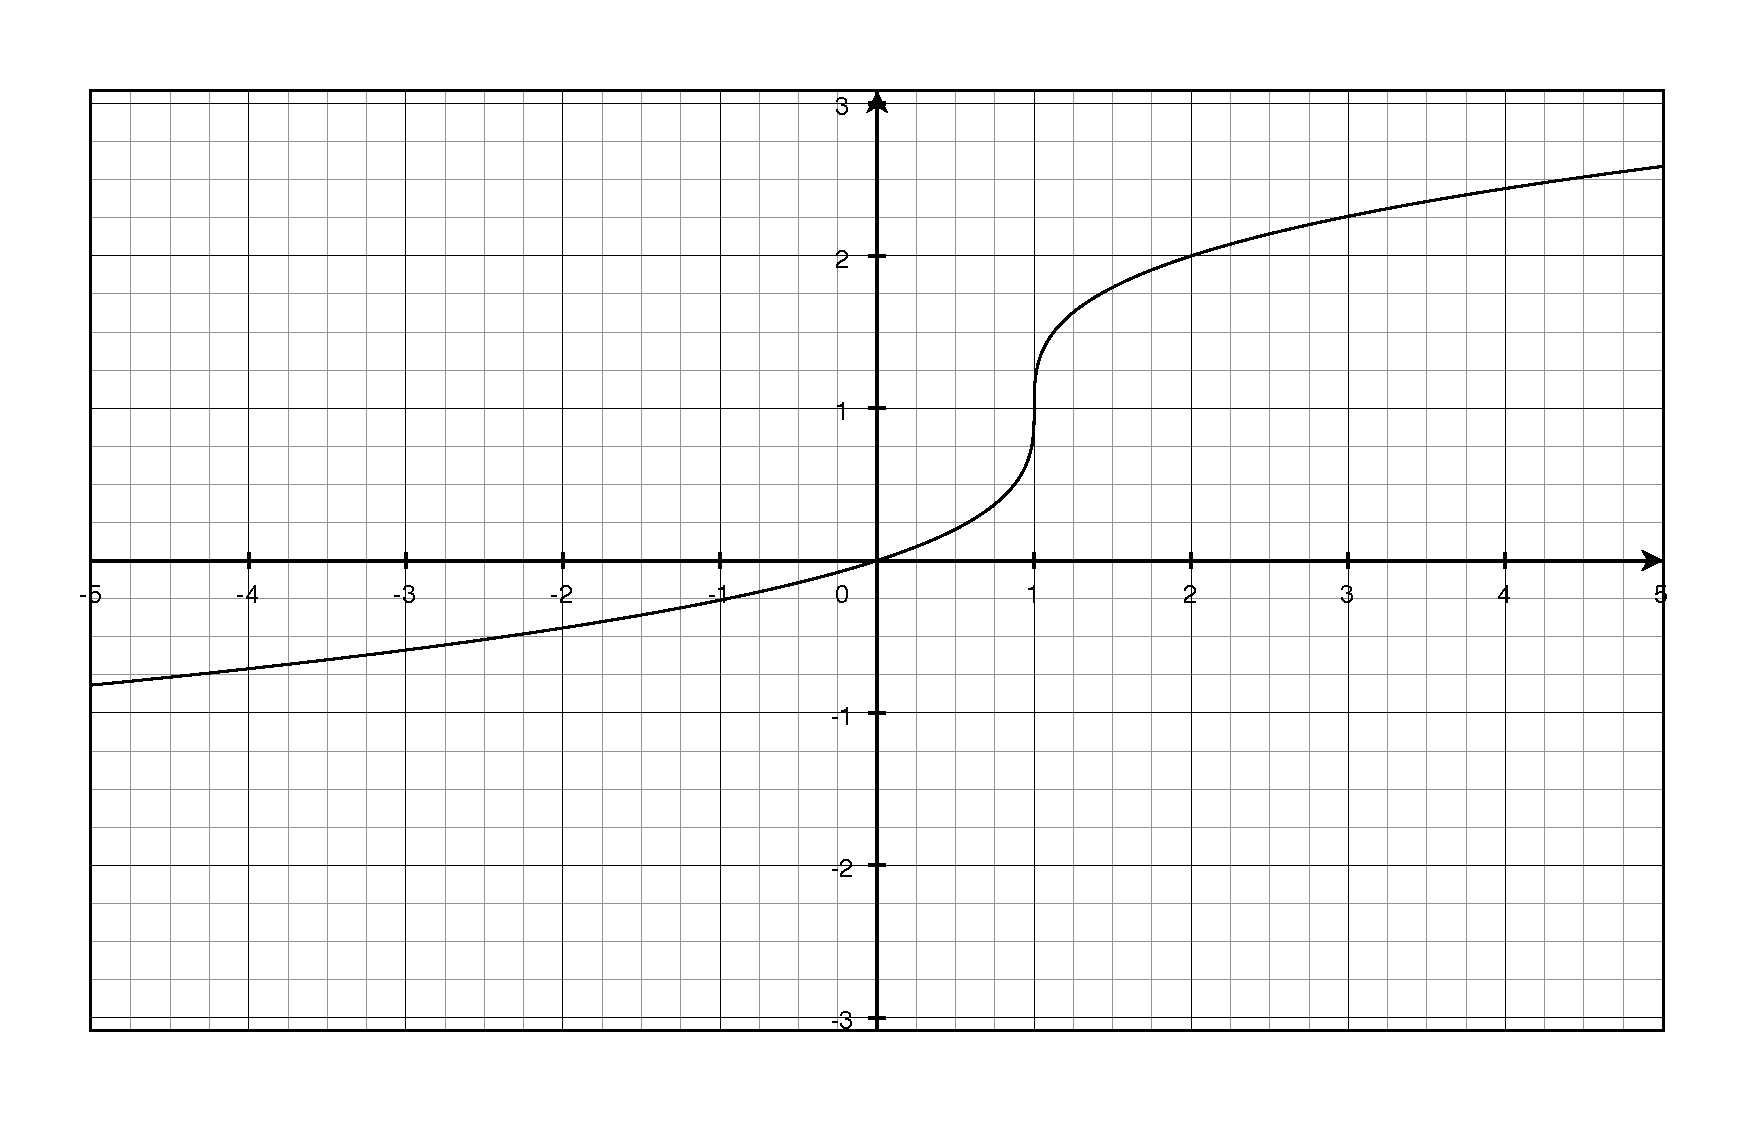
\includegraphics[scale=.3]{question7.eps}
%   \caption*{Question 7}
% \end{figure}

% \begin{tabular}{cc}
% \toprule
% period & amplitude \\
% \midrule
%   $\pi$ & $2$ \\
% \bottomrule
% \end{tabular}

\ifprintanswers
\usepackage{2in1, lscape}
\fi

\title{Math 263A Sample Final Six}

\date{November 8, 2012}

\author{}

\begin{document}

% from Fall 2010 final

\maketitle  

\begin{questions}

\question
Find the limit, if it exists. If the limit does not exist, explain why. 
\[
  \lim_{x \to 3} (2x + |x - 3|)
\]

\begin{solution}
\begin{align*}
  \lim_{x \to 3} (2x + |x - 3|) &= \lim_{x \to 3} (2x)  + \lim_{x \to 3} |x - 3| \\
  &= \lim_{x \to 3} (2x) \\
  &= 6 \\
\end{align*}
\end{solution}

\question Sketch the graph of an example function $f$ that satisfies all of the given conditions: 
\begin{itemize*}
  \item $f'(x)$ and $f''(x)$ are always negative 
  \item $f(0) = 1$
\end{itemize*}

\begin{solution}
  My computer can't draw these.
\end{solution}

\ifprintanswers
\pagebreak
\fi

\question
Prove that the equation has at least one real root: 
\[
  \cos x = x^3
\]

(Hint: graph both functions and identify an interval where a root must exist. Then use a theorem to prove it.)

\begin{solution}
Here's the graph:
\begin{figure}[H]
  \centering
  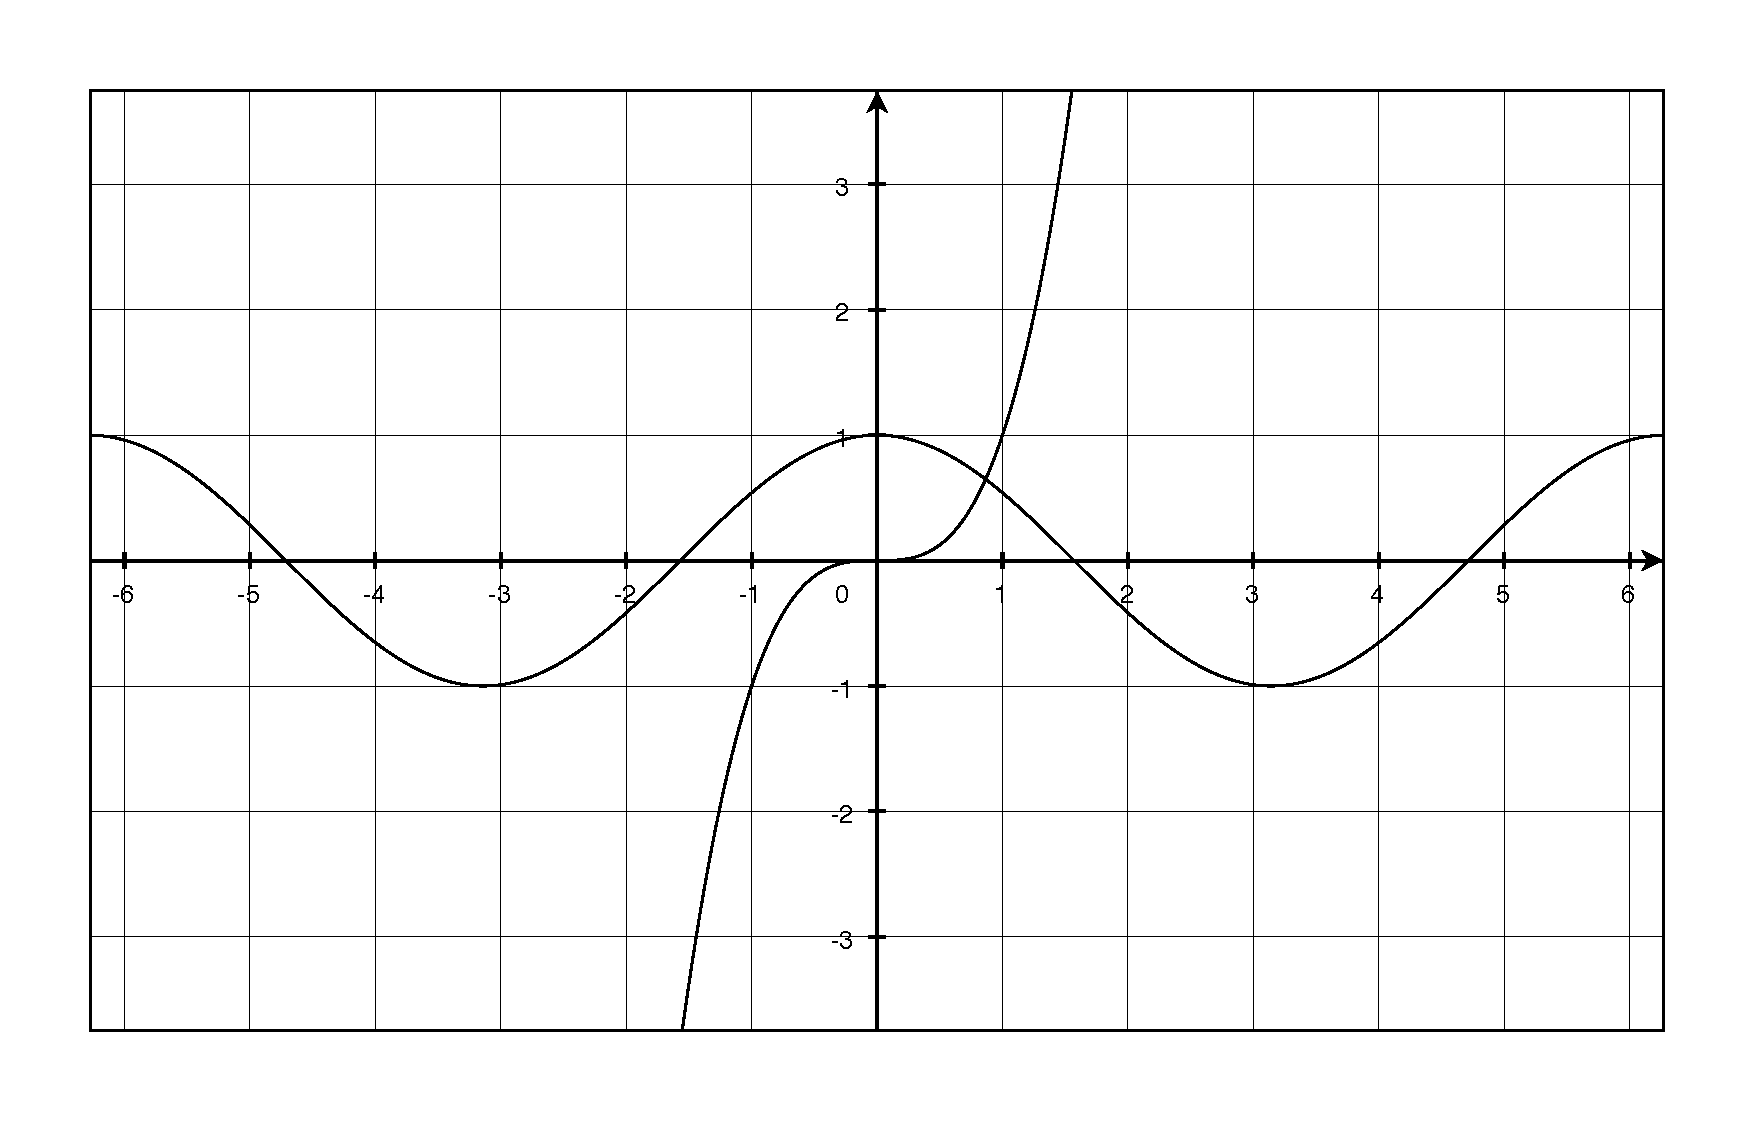
\includegraphics[scale=.3]{final_6_q3.eps}
  \caption*{Question 3}
\end{figure}

It looks like the graphs intersect somewhere between 0 and 1 and we can use the {\em Intermediate Value Theorem} to
show there is a solution.

\[
  f(x) = \cos x - x^3
\]
\begin{itemize*}
\item $f(0) = 1$
\item $f(1) = -0.46$
\end{itemize*}

Since the function must cross the x-axis between 0 and 1, there is a solution somewhere in the interval $(0, 1)$.

\end{solution}

\ifprintanswers
\pagebreak
\fi

\question $f(x) = 3x^2$
\begin{parts}
\part Find the derivative of the function using the definition of derivative. 
\begin{solution}
\begin{align*}
  f'(x) &= \lim_{h \to 0} \frac{3(x + h)^2 - 3x^2}{h} \\
        &= \lim_{h \to 0} \frac{3(x^2 + 2xh + h^2) - 3x^2}{h} \\
        &= \lim_{h \to 0} \frac{3x^2 + 6xh + 3h^2 - 3x^2}{h} \\
        &= \lim_{h \to 0} \frac{\cancel{h}(6x + 3h)}{\cancel{h}} \\
        &= \lim_{h \to 0} (6x + 3h) \\
        &= 6x \\
\end{align*}
\end{solution}

\part Check your answer using differentiation rules. 
\begin{solution}
\[
  f'(x) = 6x
\]
\end{solution}
\part State the domain of the function and the domain of the derivative.
\begin{solution}
  For both, the domain is $(-\infty, \infty)$
\end{solution}

\end{parts}

\ifprintanswers
\pagebreak
\fi

\question Find the derivatives of the functions:
\begin{parts}
\part $f(x) = (2x)^5 + 4 \pi^2$
\begin{solution}

$4 \pi^2$ is just a constant so its derivative is zero.

{\em approach 1:}
\begin{align*}
  f(x) &= (2x)^5 + 4 \pi^2 \\
       &= 32x^5 + 4 \pi^2 \\
  f'(x) &= 160x^4 \\
\end{align*}

{\em approach 2:}
\begin{align*}
  f(x) &= (2x)^5 + 4 \pi^2 \\
  f'(x) &= 5 \cdot (2x)^4 \cdot 2 \\
        &= 160x^4 \\
\end{align*}

\end{solution}

\part $g(u) = \frac{\sin u}{u^2}$
\begin{solution}
\begin{align*}
  g(u) &= \frac{\sin u}{u^2} \\
  g'(u) &= \frac{u^2 \cos u - \sin u \cdot 2u}{u^4} \\ 
        &= \frac{u \cos u - 2 \sin u}{u^3} \\ 
\end{align*}

\end{solution}

\end{parts}

\ifprintanswers
\pagebreak
\fi

\question Find the derivatives of the functions:
\begin{parts}
\part $f(t) = \frac{1}{(4t + 1)^3}$
\begin{solution}
\begin{align*}
  f(t) &= (4t + 1)^{-3} \\
  f'(t) &= -3(4t + 1)^{-4} \cdot 4 \\
        &= - \frac{12}{(4t + 1)^4} \\
\end{align*}

\end{solution}

\part $g(x) = \tan(\cos x)$
\begin{solution}
\begin{align*}
  g(x) &= \tan(\cos x) \\
  g'(x) &= \sec^2(\cos x) \cdot D_x \cos x \\
        &= - \sec^2(\cos x) \sin x \\
\end{align*}

\end{solution}

\end{parts}

\question
Find $\frac{dy}{dx}$ by implicit differentiation and simplify if possible.
\[
  \sin(x + y) = x - y
\]

\begin{solution}
\begin{align*}
  \sin(x + y) = x - y \\
  \cos(x + y)(1 + y') &= 1 - y' \\
  \cos(x + y) + y' \cos(x + y) &= 1 - y' \\
   y' + y' \cos(x + y) &= 1 - \cos(x + y) \\
   y' &= \frac{1 - \cos(x + y)}{1 + \cos(x + y)} \\
\end{align*}

\end{solution}

\question
Find the linearization (linear approximation) of the function 
\[
  f(x) = \sqrt{x}
\]
and use it to approximate the numbers $\sqrt{0.9}$ and $\sqrt{0.99}$.

\begin{solution}
Both numbers are close to 1, so we can use $dx = \{0.1, 0.01\}$ and find the corresponding $dy$s.

\begin{align*}
  y &= x^{1/2} \\
  dy &= \frac{1}{2} x^{-1/2} \, dx\\
  dy &= \frac{dx}{2 \sqrt{x}} \\
\end{align*}

For this problem, $\sqrt{x} = \sqrt{1} = 1$, so $dy = \frac{dx}{2}$, so:
\begin{align*}
  \sqrt{0.9} \approx 1 - 0.05 = 0.95 \\
  \sqrt{0.99} \approx 1 - 0.005 = 0.995 \\
\end{align*}

\end{solution}

\ifprintanswers
\pagebreak
\fi

\question
Find the derivative of the function:
\[
  g(u) = \frac{a - u}{a + u}
\]

\begin{solution}
\begin{align*}
  g'(u) &= \frac{(a + u)(-1) - (a - u)}{(a + u)^2} \\
        &= \frac{-a - u - a + u)}{(a + u)^2} \\
        &= - \frac{2a}{(a + u)^2} \\
\end{align*}

\end{solution}

\question A Norman window has the shape of a rectangle surmounted by a semicircle. (The semicircle is on top of the
rectangle and the diameter of the semicircle is the width of the rectangle.) If the perimeter of the window is to be $30
\foot$, find the dimensions of the window with the largest possible area.

\begin{solution}
If you draw a picture of the window, and use $r$ for the radius of the semicircle and $h$ for the height of the
rectangle you'll find that the perimeter and area are: 
\begin{align*}
  P &= \pi r + 2r + 2h \\
  A &= \frac{\pi r^2}{2} + 2rh \\
\end{align*}

Since we want to maximize the area, we should solve the perimeter equation for $h$ (or $r$, but $h$ seems easier) and
substitute the result in the area equation.  This gives us an area equation with only one variable.
\begin{align*}
  h &= \frac{P}{2} - \frac{\pi r}{2} - r \\
  A &= \frac{\pi r^2}{2} + 2r + 2 \left( \frac{P}{2} - \frac{\pi r}{2} - r \right) \\
    &= - \left( \frac{\pi + 4}{2} \right) r^2 + Pr \\
\end{align*}

differentiate $A$:
\[
  A' = - (\pi + 4)r + P
\]
set equal to 0 and solve:
\begin{align*}
  - (\pi + 4)r + P &= 0 \\
  r &= \frac{P}{\pi + 4} \\
\end{align*}

For our problem, $P = 30 \foot$, so $r \approx 4.2 \foot$.  Plugging this back into the height equation gives $h \approx 4.2 \foot$


\end{solution}
\question
Find the absolute maximum and minimum of the function 
\[ 
  f(x) = \sin x + \cos x
\]
on the interval $[0, \pi/3]$.

\begin{solution}
find the derivative: 
\[
  f'(x) = \cos x - \sin x
\]

find the critical point(s) in the interval:
\begin{align*}
  \cos x - \sin x &= 0 \\
  \cos x &= \sin x \\
  x &= \frac{\pi}{4} \\
\end{align*}

check for minimums and maximums

\begin{tabular}{ccc}
\toprule
$x$ & $f(x)$ & $f(x)$ approximate \\
\midrule
0                 &                      1 &       1 \\
$\frac{\pi}{4}$   &               $\sqrt{2}$ & 1.414 \\
$\frac{\pi}{3}$   & $\frac{\sqrt{3} + 1}{2}$ & 1.366 \\
\bottomrule
\end{tabular}

so the extreme points are:
\begin{itemize}
\item minimum: $(0, 1)$
\item maximum: $\left(\frac{\pi}{4}, \sqrt{2}\right)$
\end{itemize}

\end{solution}

\ifprintanswers
\pagebreak
\fi

\question
Find the critical points (critical numbers) of the function:
\[
  g(y) = \frac{y - 1}{y^2 - y + 1}
\]

\begin{solution}
\begin{align*}
  g'(y) &= \frac{y^2 - y + 1 - (y - 1)(2y - 1)}{(y^2 - y + 1)^2} \\
        &= \frac{y^2 - y + 1 - (2y^2 - 3y + 1)}{(y^2 - y + 1)^2} \\
        &= \frac{y^2 - y + 1 - 2y^2 + 3y - 1}{(y^2 - y + 1)^2} \\
        &= \frac{-y^2 + 2y}{(y^2 - y + 1)^2} \\
\end{align*}

find points where the numerator is zero:
\begin{align*}
  y(2 - y) &= 0 \\
  y &= \{0, 2\} \\ 
\end{align*}

Use the quadratic formula to find points where the denominator is zero:
\begin{align*}
  y &= \frac{1 \pm \sqrt{1 - 4}}{2} \\
    &= \frac{1 \pm i \sqrt{3}}{2} \\
\end{align*}
The solutions are both imaginary, so only the numerator points are critical points.

\end{solution}

\ifprintanswers
\pagebreak
\fi

\question
\[
  f(x) = \frac{x - 1}{x + 2}
\]

\begin{parts}
\part Find the vertical and horizontal asymptotes, if any.
\begin{solution}
Since the denominator is zero when $x = -2$, there is a vertical asymptote at $x = -2$

Since $\lim_{x \to \pm\infty} f(x) = 1$, there is a horizontal asymptote at $y = 1$

\end{solution}

\part Find the intervals on which f is increasing or decreasing. 
\begin{solution}
Find the derivative:
\begin{align*}
  f'(x) &= \frac{(x + 1) - (x - 1)}{(x + 2)^2} \\
        &= \frac{2}{(x + 2)^2} \\
\end{align*}

$f'$ is always positive so the function is increasing everywhere except where it is undefined at $x = 2$.

\end{solution}

\part Find the local maximum and minimum values of $f$.
\begin{solution}
Since the function is always increasing, there aren't any local minimums or maximums.
\end{solution}

\part Find the intervals of concavity and the inflection points. 
\begin{solution}
Find the second derivative:
\begin{align*}
  f'(x) &= 2(x + 2)^{-2} \\
  f''(x) &= -4(x + 2)^{-3} \\
         &= - \frac{4}{(x + 2)^3}
\end{align*}

$f$ is concave up on $(-\infty, -2)$ and concave down on $(2, \infty)$.

\end{solution}

\part Use the information from (a) - (d) to sketch the graph.
\begin{solution}
\begin{figure}[H]
  \centering
  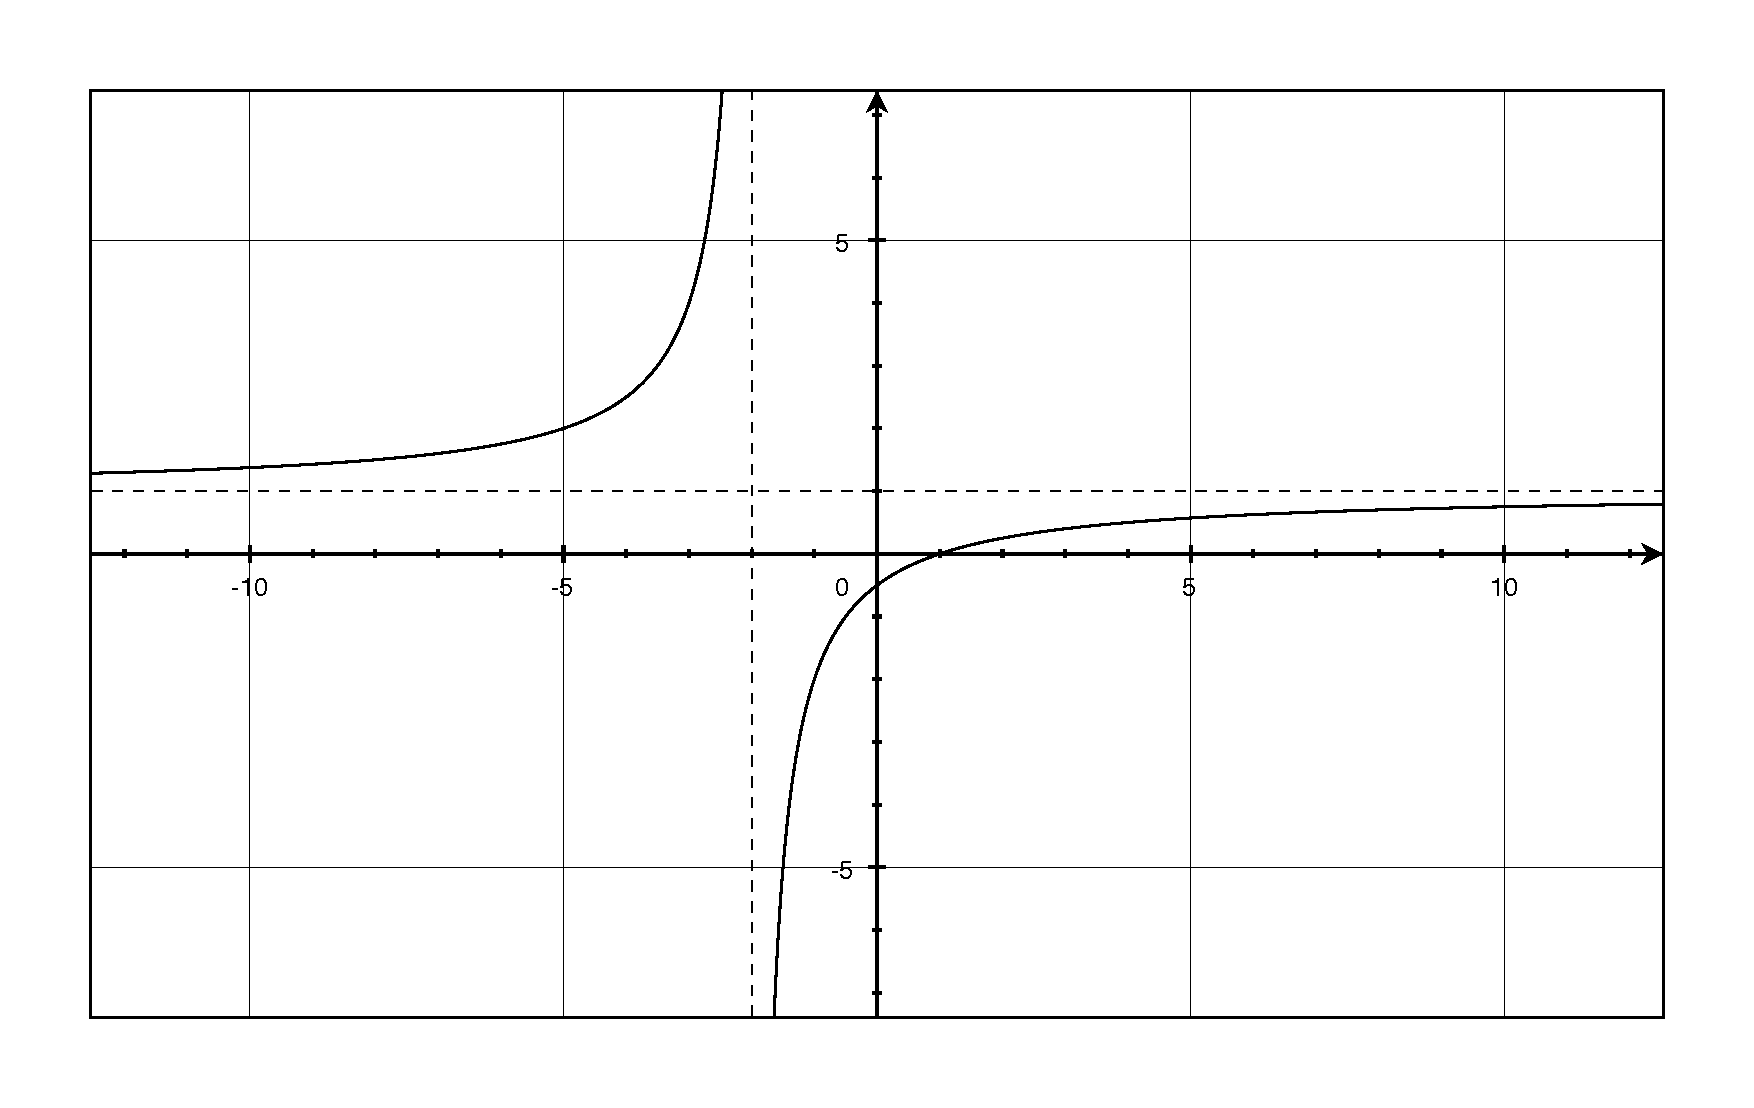
\includegraphics[scale=.3]{final_6_q13.eps}
  \caption*{Question 13}
\end{figure}

\end{solution}

\end{parts}

\end{questions}

\end{document}
